\documentclass[11pt, a4paper]{article}
\usepackage{polski}
\usepackage[utf8]{inputenc}
\usepackage[T1]{fontenc}
\usepackage[export]{adjustbox}
\usepackage{graphicx}
\usepackage{amsmath} 
\usepackage{listings}
\usepackage{color}
\usepackage{marvosym}
\usepackage{geometry}
\usepackage{enumerate}
\usepackage{float}
\usepackage{booktabs}
\usepackage{multirow}
\usepackage{titlesec}
\usepackage{hyperref}
\usepackage{tabularx}

\geometry{margin=1.2in}
\usepackage[final]{pdfpages}

\newcommand{\fbi}{\leavevmode{\parindent=1em\indent}}

\definecolor{dkgreen}{rgb}{0,0.6,0}
\definecolor{gray}{rgb}{0.5,0.5,0.5}
\definecolor{mauve}{rgb}{0.58,0,0.82}

\lstset{
	frame=tblr,
	language=R,
	aboveskip=3mm,
	belowskip=3mm,
	showstringspaces=false,
	columns=flexible,
	basicstyle={\small\ttfamily},
	numbers=left,
	numberstyle=\tiny\color{gray},
	keywordstyle=\color{blue},
	commentstyle=\color{dkgreen},
	stringstyle=\color{mauve},
	breaklines=true,
	mathescape=false,
	breakatwhitespace=true,
	tabsize=3,
	inputencoding=utf8,
	extendedchars=true,
	literate=
	{ą}{{\k{a}}}1
	{Ą}{{\k{A}}}1
	{ę}{{\k{e}}}1
	{Ę}{{\k{E}}}1
	{ó}{{\'o}}1
	{Ó}{{\'O}}1
	{ś}{{\'s}}1
	{Ś}{{\'S}}1
	{ł}{{\l{}}}1
	{Ł}{{\L{}}}1
	{ż}{{\.z}}1
	{Ż}{{\.Z}}1
	{ź}{{\'z}}1
	{Ź}{{\'Z}}1
	{ć}{{\'c}}1
	{Ć}{{\'C}}1
	{ń}{{\'n}}1
	{Ń}{{\'N}}1
}

\renewcommand\lstlistingname{Listing}

\titleclass{\subsubsubsection}{straight}[\subsection]
\newcounter{subsubsubsection}[subsubsection]
\renewcommand\thesubsubsubsection{\thesubsubsection.\arabic{subsubsubsection}}
\renewcommand\theparagraph{\thesubsubsubsection.\arabic{paragraph}}

\titleformat{\subsubsubsection}
  {\normalfont\normalsize\bfseries}{\thesubsubsubsection}{1em}{}
\titlespacing*{\subsubsubsection}
{0pt}{3.25ex plus 1ex minus .2ex}{1.5ex plus .2ex}

\makeatletter
\renewcommand\paragraph{\@startsection{paragraph}{5}{\z@}
  {3.25ex \@plus1ex \@minus.2ex}
  {-0em}
  {\normalfont\normalsize\bfseries}}
\renewcommand\subparagraph{\@startsection{subparagraph}{6}{\parindent}
  {3.25ex \@plus1ex \@minus .2ex}
  {-1em}
  {\normalfont\normalsize\bfseries}}
\def\toclevel@subsubsubsection{4}
\def\toclevel@paragraph{5}
\def\toclevel@paragraph{6}
\def\l@subsubsubsection{\@dottedtocline{4}{7em}{4em}}
\def\l@paragraph{\@dottedtocline{5}{10em}{5em}}
\def\l@subparagraph{\@dottedtocline{6}{14em}{6em}}
\makeatother

\setcounter{secnumdepth}{4}
\setcounter{tocdepth}{4}

\hypersetup{pageanchor=false}

\setlength\parindent{3pt}

\renewcommand{\labelenumi}{\alph{enumi}.} 

\date{\today}

\begin{document}

\begin{titlepage}

\newcommand{\HRule}{\rule{\linewidth}{0.5mm}} 
\center 

\textsc{\LARGE Politechnika Wrocławska}\\[1.5cm] 
\textsc{\Large Inteligencja Obliczeniowa i jej zastosowania}\\[0.5cm] 
\HRule \\[0.5cm]
{ \huge \bfseries Ćwiczenie 1: Metody redukcji wymiarowości - analiza składowych głównych}\\[0.5cm] 
\HRule \\[1.6cm]
 
\begin{minipage}{0.4\textwidth}
\begin{flushleft} \large
\emph{Autorzy:}\\
Paweł  \textsc{Andziul} 200648 \\
Robert  \textsc{Chojnacki} 200685 \\
Marcin  \textsc{Słowiński} 200638 \\
\end{flushleft}
\end{minipage}
~
\begin{minipage}{0.4\textwidth}
\begin{flushright} \large
\emph{Prowadzący:} \\
dr hab. inż. Rafał \textsc{Zdunek}
\end{flushright}
\end{minipage}\\[4cm]

\vfill 
{\large 31 maja 2017}\\[3cm] 

\end{titlepage}

\tableofcontents

\newpage
\section{Wprowadzenie}
\paragraph{}
Redukcja wymiarowości...

\fbi
Należało wykonać...

\section{Wykonane zadania}

\subsection{Zadanie 1}
\paragraph{}
Dla danych:

X = [2.5 0.5 2.2 1.9 3.1 2.3 2 1 1.5 1.1; 2.4 0.7 2.9 2.2 3 2.7 1.6 1.1 1.6 0.9];

\begin{enumerate}[a.]
\item Zaimplementować metodę PCA w Matlabie. Do wyznaczenia par własnych macierzy kowariancji można zastosować wbudowaną funkcję eig(.) lub eigs(.).
\item Wyznaczyć składowe główne i wektory cech.
\item Pokazać na rysunku punkty obserwacji oraz wyznaczone wielkości.
\end{enumerate}
\fbi
Rozwiązanie zadania polega kolejno na...

\lstinputlisting[label=lst:zad1,caption=Skrypt w Matlabie,firstline=1,lastline=500]{./assets/skrypt_zad1.m}

\begin{figure}[H]
	\centering
	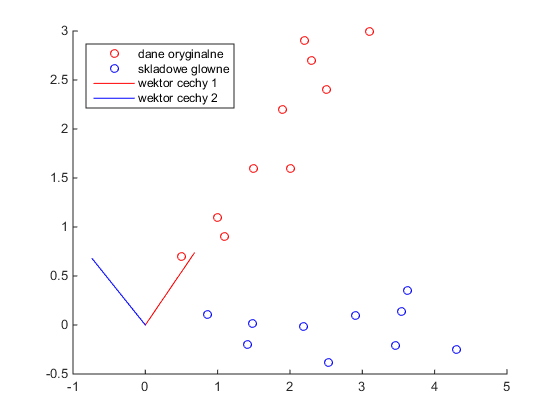
\includegraphics[width=0.95\textwidth]{./assets/ilustracja_zad1.png}
	\caption{Ilustracja punktów obserwacji i składowych głównych}
	\label{fig:zad1}
\end{figure}

\fbi
Z wykresu można...

\subsection{Zadanie 2}
\paragraph{}
Dla obrazów twarzy z bazy ORL (lub podobnej) wyznaczyć cechy holistyczne (twarze własne) dla różnej liczby estymowanych komponentów głównych (J = 4, 10, 20, 30). Pogrupować obrazy stosując metodę k-średnich, do obrazów oryginalnych oraz redukowanych. Badania przeprowadzić dla różnej liczby grup. Porównać dokładność i czas grupowania. Następnie dokonać klasyfikacji obrazów w obu przestrzeniach (oryginalnej i zredukowanej) za pomocą klasyfikatora k-NN. Porównać efekty klasyfikacji z efektami grupowania.

\fbi
Skrypt...

\subsection{Zadanie 3}
\paragraph{}
Wyznaczyć pary własne macierzy kowariancji za pomocą algorytmów: Powera oraz Lanczosa. Zaimplementować algorytmy i zastosować je do rozwiązania powyższych zadań. Porównać wyniki.



\section{Podsumowanie}
\paragraph{}
W trakcie przeprowadzonych badań...

\newpage
\begin{thebibliography}{40}

\bibitem{test1}
\url{https://www.mathworks.com/help/nnet/ref/plotconfusion.html}

\bibitem{test2}
\url{https://www.mathworks.com/help/stats/confusionmat.html}

\bibitem{test3}
\url{https://en.wikipedia.org/wiki/Lanczos_algorithm}

\bibitem{test4}
\url{http://www.kmg.zut.edu.pl/opt/wyklad/bezgrad/powell.html}

\end{thebibliography}

\end{document}
